%%%%%%%%%%%%%%%%%%%%%%%%%%%%%%%%%%%%%%%%%%%%%%%%%%%%%%%%%%%%%%%%%%%%%%%%%%%%%%%%%%%%%%%%%%%%%%%%%
%%%%%  Beamer Sildes  %%%%%%%%%%%%%%%%%%%%%%%%%%%%%%%%%%%%%%%%%%%%%%%%%%%%%%%%%%%%%%%%%%%%%%%%%%%
%%%%%%%%%%%%%%%%%%%%%%%%%%%%%%%%%%%%%%%%%%%%%%%%%%%%%%%%%%%%%%%%%%%%%%%%%%%%%%%%%%%%%%%%%%%%%%%%%

% https://en.wikibooks.org/wiki/LaTeX/Presentations

\documentclass{beamer}
% \mode<presentation> {
\mode<handout> {

    %%%%%  Themes  %%%%%%%%%%%%%%
    %%%%%%%%%%%%%%%%%%%%%%%%%%%%%
    % \usetheme{AnnArbor}
    % \usetheme{Antibes}
    % \usetheme{Bergen}
    % \usetheme{Berkeley}
    % \usetheme{Berlin}
    % \usetheme{CambridgeUS}
    % \usetheme{Copenhagen}
    % \usetheme{Darmstadt}
    % \usetheme{Dresden}
    % \usetheme{Frankfurt}
    % \usetheme{Goettingen}
    % \usetheme{Hannover}
    % \usetheme{Ilmenau}
    % \usetheme{JuanLesPins}
    % \usetheme{Luebeck}
    % \usetheme{Madrid}
    % \usetheme{Malmoe}
    % \usetheme{Marburg}
    % \usetheme{Montpellier}
    % \usetheme{PaloAlto}
    % \usetheme{Pittsburgh}
    % \usetheme{Rochester}
    % \usetheme{Singapore}
    % \usetheme{Szeged}
    % \usetheme{Warsaw}
    % \usetheme{boxes}
    \usetheme{default}

    %%%%%  Color Themes  %%%%%%%%
    %%%%%%%%%%%%%%%%%%%%%%%%%%%%%
    % \usecolortheme{default}
    % \usecolortheme{albatross}
    % \usecolortheme{beaver}
    % \usecolortheme{beetle}
    % \usecolortheme{crane}
    % \usecolortheme{dolphin}
    % \usecolortheme{dove}
    % \usecolortheme{fly}
    % \usecolortheme{lily}
    % \usecolortheme{orchid}
    % \usecolortheme{rose}
    % \usecolortheme{seagull}
    % \usecolortheme{seahorse}
    % \usecolortheme{whale}
    % \usecolortheme{wolverine}

    %%%%%  Outer Themes  %%%%%%%%
    %%%%%%%%%%%%%%%%%%%%%%%%%%%%%
    % \useoutertheme{infolines}
    % \useoutertheme{miniframes}
    % \useoutertheme{shadow}
    % \useoutertheme{sidebar}
    % \useoutertheme{smoothbars}
    % \useoutertheme{smoothtree}
    % \useoutertheme{split}
    % \useoutertheme{tree}

    %%%%%  Inner Themes  %%%%%%%%
    %%%%%%%%%%%%%%%%%%%%%%%%%%%%%
    % \useinnertheme{rectangles}
    % \useinnertheme{circles}
    % \useinnertheme{inmargin}
    % \useinnertheme{rounded}
}

\usepackage{amsthm}
\usepackage{amsmath}
\usepackage{amssymb}
\usepackage{array}
\usepackage[fleqn]{mathtools}
\usepackage{caption}
\usepackage{wallpaper}
\usepackage{xcolor}
\definecolor{umblue}{HTML}{00274C}
\definecolor{ummaize}{HTML}{FFCB05}
\usepackage{colortbl}
\usepackage{graphicx} 
\usepackage{pgf}
\usepackage{tikz}
\usetikzlibrary{arrows,automata}
\usepackage{url}			       
\usepackage{hyperref}

% \setbeamercolor{alerted text}{fg=orange}
% \setbeamercolor{background canvas}{bg=white}
% \setbeamercolor{block body alerted}{bg=normal text.bg!90!black}
% \setbeamercolor{block body}{bg=normal text.bg!90!black}
% \setbeamercolor{block body example}{bg=normal text.bg!90!black}
% \setbeamercolor{block title alerted}{use={normal text,alerted text},fg=alerted text.fg!75!normal text.fg,bg=normal text.bg!75!black}
% \setbeamercolor{block title}{bg=blue}
% \setbeamercolor{block title example}{use={normal text,example text},fg=example text.fg!75!normal text.fg,bg=normal text.bg!75!black}
% \setbeamercolor{fine separation line}{}
\setbeamercolor{frametitle}{fg=umblue}
\setbeamercolor{item projected}{fg=umblue}
% \setbeamercolor{normal text}{bg=black,fg=yellow}
% \setbeamercolor{palette sidebar primary}{use=normal text,fg=normal text.fg}
% \setbeamercolor{palette sidebar quaternary}{use=structure,fg=structure.fg}
% \setbeamercolor{palette sidebar secondary}{use=structure,fg=structure.fg}
% \setbeamercolor{palette sidebar tertiary}{use=normal text,fg=normal text.fg}
% \setbeamercolor{section in sidebar}{fg=brown}
% \setbeamercolor{section in sidebar shaded}{fg=grey}
% \setbeamercolor{separation line}{}
% \setbeamercolor{sidebar}{bg=red}
% \setbeamercolor{sidebar}{parent=palette primary}
% \setbeamercolor{structure}{bg=ummaize, fg=umblue}
% \setbeamercolor{subsection in sidebar}{fg=brown}
% \setbeamercolor{subsection in sidebar shaded}{fg=grey}
\setbeamercolor{title}{fg=umblue}
% \setbeamercolor{titlelike}{fg=umblue}

% \setbeamertemplate{page number in foot}[appendixframenumber]
\setbeamertemplate{footline}[frame number]
% \setbeamertemplate{blocks}[rounded][shadow=true]
% \setbeamertemplate{background canvas}[vertical shading][bottom=white,top=structure.fg!25]
% \setbeamertemplate{sidebar canvas left}[horizontal shading][left=white!40!black,right=black]
\setbeamertemplate{itemize item}{\color{umblue}$\blacktriangleright$}
\setbeamertemplate{itemize subitem}{\color{umblue}$\ast$}

\setbeamerfont*{footline}{family=\sffamily, size=\large}
% \setbeamerfont{title}{family=\rmfamily\addfontfeatures{Scale=1.18, Numbers={Lining, Proportional}}}
\usefonttheme[onlymath]{serif}

\beamertemplatenavigationsymbolsempty

\hypersetup{pdfstartview={Fit}} % fits the presentation to the window when first displayed

\newcommand{\XB}{\color{black}}
\newcommand{\XBB}{\color{blue}}
\newcommand{\XV}{\color{violet}}
\newcommand{\XR}{\color{red}}
\newcommand{\XUMB}{\color{umblue}}
\newcommand{\XUMM}{\color{ummaize}}

\newcommand{\ds}{\displaystyle}

% Use pause in math enviornments
\makeatletter
\renewrobustcmd{\beamer@@pause}[1][]{
  \unless\ifmeasuring@
  \ifblank{#1}
    {\stepcounter{beamerpauses}}
    {\setcounter{beamerpauses}{#1}}
  \onslide<\value{beamerpauses}->\relax
  \fi
}
\makeatother

%%%%%%%%%%%%%%%%%%%%%%%%%%%%%%%%%%%%%%%%%%%%%%%%%%%%%%%%%%%%%%%%%%%%%%%%%%%%%%%%%%%%%%%%%%%%%%%%%
%%%%%  Title Page  %%%%%%%%%%%%%%%%%%%%%%%%%%%%%%%%%%%%%%%%%%%%%%%%%%%%%%%%%%%%%%%%%%%%%%%%%%%%%%
%%%%%%%%%%%%%%%%%%%%%%%%%%%%%%%%%%%%%%%%%%%%%%%%%%%%%%%%%%%%%%%%%%%%%%%%%%%%%%%%%%%%%%%%%%%%%%%%%

\title[Short Title]{Long Title}
\author{\XV\textit{\large{\href{https://github.com/casonk}{Cason Konzer}}}\XB}
\institute[UM FLINT]{\normalsize{\textit{\href{mailto:casonk@umich.edu}{casonk@umich.edu}}}}
\titlegraphic{\includegraphics[scale = 0.5]{C:/Users/cason/OneDrive - Umich/TeMpLaTeX/University_of_Michigan_Flint.png}}
\date[]{\today} 

\begin{document}

\begin{frame}
    \titlepage
\end{frame}


%%%%%%%%%%%%%%%%%%%%%%%%%%%%%%%%%%%%%%%%%%%%%%%%%%%%%%%%%%%%%%%%%%%%%%%%%%%%%%%%%%%%%%%%%%%%%%%%%
%%%%%  Begin Slides  %%%%%%%%%%%%%%%%%%%%%%%%%%%%%%%%%%%%%%%%%%%%%%%%%%%%%%%%%%%%%%%%%%%%%%%%%%%%
%%%%%%%%%%%%%%%%%%%%%%%%%%%%%%%%%%%%%%%%%%%%%%%%%%%%%%%%%%%%%%%%%%%%%%%%%%%%%%%%%%%%%%%%%%%%%%%%%

%%%%%  Introduction  %%%%%%%%%%%%%%%%%%%%%%%%%%%%%%%%%%%%%%%%%%%%%%%%%%%%%%%%%%%%%%%%%%%%%%%%%%%%

\section{Introduction}

\begin{frame}

    \frametitle{Introduction}

    Simple List \pause

    \vspace{2.5mm}
    \begin{itemize}
        \item Item.\pause
        \begin{itemize}
            \item Sub Item.\pause
        \end{itemize}
    \end{itemize}

\end{frame}

%%%%%  SectName  %%%%%%%%%%%%%%%%%%%%%%%%%%%%%%%%%%%%%%%%%%%%%%%%%%%%%%%%%%%%%%%%%%%%%%%%%%%%%

\begin{frame}

    \frametitle{Image}
    \includegraphics[width=\textwidth]{C:/Users/cason/OneDrive - Umich/TeMpLaTeX/University_of_Michigan_Flint.png}

\end{frame}


\begin{frame}

    \frametitle{Allignment 1}

    \begin{flalign*}
        & \ds \sum_{i, j}^{n} \mathbb{E}_{i, j} = \sum_{i, j \ne i}^{n} \mathbb{E}_{i, j} + \sum_{i}^{n} \mathbb{E}_{i, i} \\ \pause
        &= \sum_{i, j \ne i}^{n} \frac{k_{i} k_{j}}{s - 1} + \sum_{i}^{n} \frac{k_{i} (k_{i} - 1)}{s - 1} \\ \pause
        &= \frac{1}{s - 1} \left[ \sum_{i}^{n} k_{i} \sum_{j \ne i}^{n} k_{j} + \sum_{i}^{n} k_{i} \sum_{i}^{n} k_{i} - \sum_{i}^{n} k_{i} \right] \\ \pause
        &= \frac{1}{s - 1} \left[ \sum_{i}^{n} k_{i} \sum_{j}^{n} k_{j} - s \right] \\ \pause
        &= \frac{s^{2} - s}{s - 1} \pause = \frac{s(s - 1)}{s - 1} \pause = s
    \end{flalign*}

\end{frame}

\begin{frame}

    \frametitle{Allignment 2}

    \begin{flalign*}
        & \ds \sum_{i, j}^{n} \vec{\mathbb{E}}_{i, j} = \sum_{i, j}^{n} \frac{k_{i}^{out} k_{j}^{in}}{m} \\ \pause
        &= \frac{1}{m} \left[ \sum_{i}^{n} k_{i}^{out} \sum_{j}^{n} k_{j}^{in} \right] \\ \pause
        &= \frac{m^{2}}{m} \pause = m
    \end{flalign*}

\end{frame}

%%%%%  SectName  %%%%%%%%%%%%%%%%%%%%%%%%%%%%%%%%%%%%%%%%%%%%%%%%%%%%%%%%%%%%%%%%%%%%%%%%%%%%%%%

\section{SectName}

\begin{frame}

    \frametitle{Cases}

    \vspace{2.5mm}
    \begin{itemize}
        \item $ Q = \% \ internal \ edges - Expected \ \% \ internal \ edges $.\pause
        \item $ \ds \delta(c_{i}, c_{j}) =
            \begin{cases}
                1 & i \ \& \ j \ are \ in \ the \ same \ community \\ \pause
                0 & else
            \end{cases}
            $.\pause
        \item Note: $ \delta(c_{i}, c_{i}) = 1 $.\pause
    \end{itemize}

    \vspace{2.5mm}
    \begin{multline*}
        \ds Q = \frac{1}{s} \Biggl[ \sum_{i, j \ne i}^{n} \left( A_{i, j} - \frac{k_{i}k_{j}}{s - 1} \right) \delta(c_{i}, c_{j}) \\ 
        +  \sum_{i}^{n} \left( A_{i,i} - \frac{k_{i}(k_{i} - 1)}{s - 1} \right) \Biggr].
    \end{multline*}

\end{frame}

%%%%%  Algorithms  %%%%%%%%%%%%%%%%%%%%%%%%%%%%%%%%%%%%%%%%%%%%%%%%%%%%%%%%%%%%%%%%%%%%%%%%%%%%%%%

\section{Algorithms}


\begin{frame}

    \frametitle{Algorithms}


\end{frame}

%%%%%  Examples

\tikzset{every loop/.style={min distance=5mm}}
\begin{frame}

    \frametitle{TikZ}
    \begin{figure}[t]
        \centering
        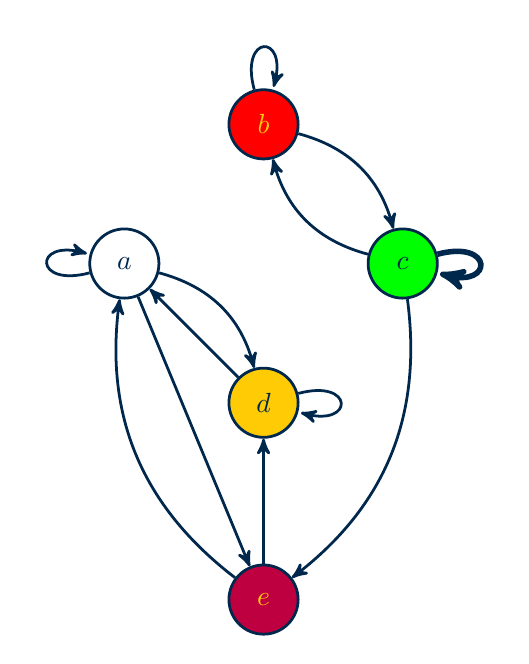
\begin{tikzpicture}[->,>=stealth',auto,node distance=2.5cm,semithick,line width=1pt]
            \tikzstyle{be}=[color=umblue]
            \tikzstyle{be2}=[color=umblue,line width=2pt]
            
            \node[state,fill=white,draw=umblue,text=umblue]   (A)                    {$a$};
            \node[state,fill=red,draw=umblue,text=ummaize]    (B) [above right of=A] {$b$};
            \node[state,fill=ummaize,draw=umblue,text=umblue] (D) [below right of=A] {$d$};
            \node[state,fill=green,draw=umblue,text=umblue]   (C) [below right of=B] {$c$};
            \node[state,fill=purple,draw=umblue,text=ummaize] (E) [below of=D]       {$e$};
            
            \path   (A) edge [be,loop  left]   node {} (A)
                        edge [be]              node {} (E)
                        edge [be, bend left]   node {} (D)
                    (B) edge [be, loop above]  node {} (B)
                        edge [be, bend  left]  node {} (C)
                    (C) edge [be2, loop right] node {} (C)
                        edge [be, bend  left]  node {} (E)
                        edge [be, bend  left]  node {} (B)
                    (D) edge [be, loop right]  node {} (D)
                        edge [be]              node {} (A)
                    (E) edge [be, bend  left]  node {} (A)
                        edge [be]              node {} (D);
            
        \end{tikzpicture}
    \end{figure}  

\end{frame}

\begin{frame}

    \frametitle{Matrix}

    \begin{center}
        \begin{tabular}{l | c c c c c} 
            $ \vec{A} $ & $ a $ & $ b $ & $ c $ & $ d $ & $ e $ \\
            \hline
            $ a $ & $ 1 $ & $ 0 $ & $ 0 $ & $ 1 $ & $ 1 $ \\
            $ b $ & $ 0 $ & $ 1 $ & $ 1 $ & $ 0 $ & $ 0 $ \\
            $ c $ & $ 0 $ & $ 1 $ & $ 2 $ & $ 0 $ & $ 1 $ \\
            $ d $ & $ 1 $ & $ 0 $ & $ 0 $ & $ 1 $ & $ 0 $ \\
            $ e $ & $ 1 $ & $ 0 $ & $ 0 $ & $ 1 $ & $ 0 $ \\
        \end{tabular}
    \end{center}\pause

    \vspace{2.5mm}
    The adjacency matrix is the expected form computers will store networks in. 

\end{frame}

\begin{frame}

    \frametitle{Colored Table}

    Colored Table
    \begin{center}
        \begin{tabular}{l | c c c c} 
            $ merge    $ & $ \partial \vec{Q}_{i} $ & $ \partial \vec{Q}_{j} $ & $ \partial \vec{Q}_{i'} $ & $ \Delta \vec{Q} $ \\
            \hline
            \rowcolor{ummaize}
            $ \{a, d\} $ & $ 4/13  $ & $  7/13  $ & $ 22/13 $ & $ 11/169 $ \\
            \rowcolor{ummaize}
            $ \{a, e\} $ & $ 4/13  $ & $ -4/13  $ & $ 14/13 $ & $ 14/169 $ \\
            \rowcolor{ummaize}
            $ \{b, c\} $ & $  9/13 $ & $  14/13 $ & $ 35/13 $ & $ 12/169 $ \\
            $ \{c, e\} $ & $ 14/13 $ & $ -4/13  $ & $  9/13 $ & $ -1/169 $ \\
            $ \{d, e\} $ & $  7/13 $ & $ -4/13  $ & $  6/13 $ & $  3/169 $ \\
        \end{tabular}
    \end{center}\pause

    \vspace{2.5mm}
    The best merge for nodes $ a $, and $ e $, is to merge them together, similarly, the best for $ b $, and $ c $, is to merge them together, last, the best merge for $ d $ is to merge it with $ a $. 

\end{frame}

%%%%%  Conclusion  %%%%%%%%%%%%%%%%%%%%%%%%%%%%%%%%%%%%%%%%%%%%%%%%%%%%%%%%%%%%%%%%%%%%%%%%%%%%%%%

\section{Conclusion}

\begin{frame}
    \frametitle{Conclusion}

    We truly covered a lot, and yet this is only a glimpse.\pause

    \hrulefill \\
    \Large{\centerline{\XR QUESTIONS?\XB}} 
    \normalsize{\centerline{\textit{\href{mailto:casonk@umich.edu}{casonk@umich.edu}}}}

\end{frame}

\begin{frame}
    \frametitle{References [1/4]}

    [1] Arenas, A., Fern{\'{a}}ndez, A., and G{\'{o}}mez, S.
    Analysis of the structure of complex networks at
    different resolution levels. New Journal of Physics 10, 5
    (May 2008). \\

    [2] Barab{\'{a}}si, A. L. Network Science. Cambridge
    University Press, 2016. \\

    [3] Blondel, V. D., Guillaume, J.-L., Lambiotte, R.,
    and Lefebvre, E. Fast unfolding of communities in
    large networks. Journal of Statistical Mechanics: Theory
    and Experiment (Oct. 2008).

    [4] Dugu{\'{e}}, N., and Perez, A. Directed Louvain :
    maximizing modularity in directed networks. Research
    report, Universit{\'{e}} d'Orl{\'{e}}ans, Nov. 2015. \\

    [5] Girvan, M., and Newman, M. E. J. Community
    structure in social and biological networks. Proceedings
    of the National Academy of Sciences 99, 12 (2002),
    7821–7826.

\end{frame}

\end{document} 

